% siminos/xiong/thesis/proposal/tex/intro.tex
% $Author: predrag $ $Date: 2017-03-06 17:13:44 -0500 (Mon, 06 Mar 2017) $

\section{Introduction}
\label{sec:Intro}

\subsection{\CycForm s}
Statistical properties and geometrical structure are among the major
questions in the study of chaotic nonlinear dissipative systems.
Generally,
such a system will get trapped to a invariant set,
which is called global
(maximal) attractor after a transient period, and we are only interested
in the dynamics on the attractor, especially the temporal
physical quantities such as average diffusion rate, energy dissipation rate,
Lyapunov exponents and so on. The intrinsic instability of
orbits on the attractor make the long time simulation unreliable, which is
also time consuming. According to the ergodic theorem\rf{EckmannRuelle1985}, %eckerg},
long time averaging converges to the same answer as a spatial average over the attractor, provided
we know the natural measure on the attractor. However, as a strange attractor usually has
support on a fractal structure, and a non-continuous measure, such computations
are not numerically feasible. This is where the \po\ theory\rf{DasBuch} enters.
Invariant subset accompanied with their stable/unstable manifolds shape
the orbits on global attractor. Usually, we can find a few \eqva\ (or relative
\eqva\ if system possesses continuous symmetries), and a dense, zero measure set of
(relative) \po s. Predecessors proved a direct link between
a weighted sum of physical quantities on \po s and the long time averages
in the form of \emph{\Fd}\rf{CBconverg}
\beq
    \det(\eigenvL - \Aop)  \defeq \exp \left(
        - {
    \sum_{p} \sum_{r=1}^\infty \frac{1}{r}
        \frac{   e^{r (\beta \Obser_p -\eigenvL\period{p}) }}
             {\oneMinJ{r}}
            }\right)
    \,,
    \label{Z(s)}
\eeq
where subscript $p$ denote the \po s, $M_p$ is the {\monodromyM}
along a \po, $A_p$ is the physical observable integrated along the
orbit $\Obser(\xInit,t) =\int_0^t d\tau \, \obser(\ssp(\tau))$
and $T_p$ is the period. The largest zero point $\eigenvL(\beta)$ of
\eqref{Z(s)} is a implicit function of parameter $\beta$, and it is claimed that
average of $a(\ssp(t))$ is given by
\begin{equation}
  \label{eq:expect}
  \left.\frac{\partial \eigenvL}{\partial \beta_j}
  \right|_{\beta=0} = \expct{\obser_j}
\end{equation}
Note, the above sum involves the summation of all \po s inside this system.
In
practice, we truncate \eqref{Z(s)} according to the topological length of \po s,
which is primarily established by symbolic dynamics, or if not available, by
stability of \po s. This technique is called \emph{cycle expansion},
whose effectiveness has been demonstrated in a few 1-dimensional maps\rf{AACI, AACII} and
ergodic flows \rf{BuBoCvSi14, Christiansen97, lanCvit07}.


\subsection{Inertial manifold}
\label{subsec:IM}
Symbolic dynamics provides a complete topological description on the attractor.
However, in practice, it is difficult to extract such simplified dynamics on
strange attractor, especially
for high dimensional turbulent flows. Also, other geometric properties are
interesting but beyond the capability of symbolic dynamics. One such property is
the effective dimension of attractor. For dissipative systems, global attractor
is a measure-zero invariant subset of the state space concerned, and usually has non-smooth
surface and fractal dimension, which make it hard to analyze, so we wish to
use a `tight' smooth manifold that encloses it but has nicer properties. This
is called \emph{inertial manifold}\rf{Foias1988a, infdymnon}.
These two concepts are different mainly by their
local properties. Each point on inertial manifold with
its neighborhood behaves as $\mathbb{R}^M$ ( homeomorphic to an
open subset
of $\mathbb{R}^M$) with integer number $M$ the dimension of inertial manifold.
For a strange attractor, the scenario is much more complicated. Also, we need
to
explain the meaning of `tight'. It refers to the fact that it is a
forward invariant manifold with
lowest dimension that encloses the global attractor and attracts
points in the state
space exponentially fast.

The existence of global attractor and/or inertial manifold has been proved
for many chaotic or turbulent systems\rf{infdymnon}. Also
numerical methods
such as Euler-Galerkin\rf{foias88}, nonlinear Galerkin method\rf{Marion1989} to approximate
inertial manifold have been proposed, but the discussion of
all these methods focuses on the performance over standard Galerkin method.
Little is known about the exact dimension of
inertial manifold except a few systems\rf{infdymnon}.
For our interest in 1-dimensional \KSe, only upper bound,
to the best knowledge of the author, is given as
proportional to $L^{2.46}$\rf{jolly_evaluating_2000, Robinson-PLA1994},
which is far above our linear relation
expectation in spatiotemporal chaos.

On the other hand, the progress
in numerical method to calculate \emph{\cLv}s\rf{GiChLiPo12, KuPa12}
motivated physicists to
try to expand inertial manifold by
\cLvs\ locally through statistical study of the tangency among
\cLvs\ \rf{YaTaGiChRa08} and
difference vector projection\rf{YaRa11}. The number of the \cLvs\ needed
for a faithful expansion is
regarded as the dimension of inertial manifold. The key observation
in this study is that tangent space can be decomposed of an
entangled physical subspace and a contracting disentangled subspace,
and the latter is thought to be irrelevant to the long time behavior
on the inertial manifold.
Similar properties have been observed on \Fv s
associated with \po s inside \KSe, so we expect to get
the same result about the dimension of inertial manifold by focusing
on \po s instead of a long ergodic trajectory.
Also, our work focuses on the continuous symmetry reduced space,
whose inertial manifold is one dimension less than that in the original
space.

\subsection{Covariant algorithm and \psd}
\label{subsec:CAPSD}
Physicists are trying to understand dynamical systems by
topological invariant objects inside these systems,
such as \eqva,
\po s, invariant tori, etc. For instance,
The \emph{multiplicative ergodic theorem} (Oseledets theorem)\rf{lyaos, ruelle79}
states that
there is an forward and backward invariant subspace $W_i(x)$
associated with each Lyapunov exponent $\Lyap_i$ in dynamical systems.
\begin{equation}
  \label{eq:lyapunov}
  \lim_{t\to\pm\infty}\frac{1}{|t|}\ln\norm{J^t(x)u}
  = \pm\Lyap_i
  \,,\quad  u\in W_i(x)
\end{equation}
If a Lyapunov exponent has degeneracy one, the corresponding
subspace $W_i(x)$ reduces to a vector, called \emph{\cLv}.
This statement dates back to 1960's, but the
corresponding numerical algorithms are invented quite recently, which
is also the basis of the work on investigating the dimension of inertial
manifold mentioned in sec.~\ref{subsec:IM}.
Our \Fv\ algorithm in sec.~\ref{subsec:PE} is motivated by
\cLv\ algorithm. Also,
for \po s, $\Lyap_i$ coincide with the real part of Floquet exponents,
and subspace $W_i(x)$ coincides with
a \Fv, or, if there is degeneracy, a subspace
spanned by the degenerate \Fv s.

Another algorithm, \psd\rf{Bojanczyk92theperiodic},
is also the basis of our \Fv\
algorithm. This algorithm enables us to calculate the eigenvalues
of the product of a sequence of square matrices without forming the
product it explicitly. This scenario happens in the stability analysis
of \po s in dynamical system since {\monodromyM} follows
the chain rule and thus can be decomposed as the product of a sequence
of matrices. We should mention that \psd\ transforms individual
matrices into upper-triangular or quasi-upper triangular form,
so eigenvalues are manifest as the product of diagonal elements of all
these matrices; however, to obtain the corresponding eigenvectors or
a subset of eigenvectors, we need to take further steps based on
\psd, which is illustrated in sec.~\ref{subsec:PE}.

\subsection{Intermittent explosion in \cqcGLe}
\label{subsec:cqcgl}

Derived as a general amplitude equation near bifurcation point,
\cGLe\rf{cross93} has ubiquitous applications
in various areas of physics,
and serves as a prototype for a lot of other equations such as
nonlinear Schr\"odinger equation. Its cubic form is
frequently used to study turbulence and intermittent traveling
waves. But, recently, \cGLe\ with a cubic quintic nonlinear term attracts
much attention for its peculiar intermittent explosion of soliton solution
in one dimensional and two dimensional cases. Here, we focus on
the one dimensional quintic complex Ginzburg-Landau equation defined
on a periodic domain
\begin{equation}
  \label{eq:cqcgl1d}
  A_t = \mu A + DA_{xx} + \beta |A|^2A + \gamma |A|^4A \,,\quad x\in[0,L]
  \,.
\end{equation}
Here, $A(x,t)$ is a complex field. Coefficient $\mu$ is real and
the other three coefficients are complex.
\[
D = D_r + iD_i\,,\quad \beta = \beta_r + i\beta_i\,,\quad
\gamma = \gamma_r + i\gamma_i
\,.
\]
Parameters are fixed to $D=0.125+0.5i$, $\beta=1+0.8i$, $\gamma=-0.1-0.6i$,
$L=50$ .

Since $\beta$ has positive real part, \cqcGLe\ undergoes subcritical
bifurcation at $\mu=0$.  Moreover, as shown in
\refref{Deissler1994}, increasing
$\mu$ from very negative to zero, the system undergoes stable pulses,
oscillating pulses with one frequency, pulses with two frequency, and
symmetric/asymmetric explosion. We set $\mu=-0.213$
the same as in \refrefs{Descalzi10,Jaime2012,Jaime2013,Akhmediev04}
to observe symmetric and
asymmetric explosion as shown in \reffig{fig:explosionTypes}.

\begin{figure}[h]
  \centering
  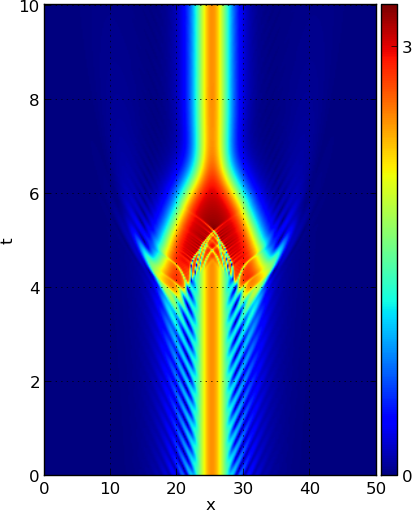
\includegraphics[width=0.33\textwidth]{symmetricExplosion}%\hfill
  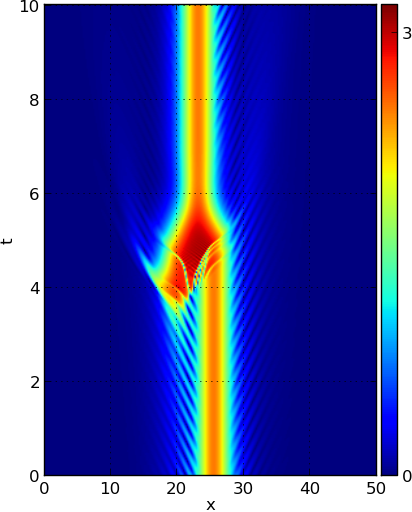
\includegraphics[width=0.33\textwidth]{asymmetricExplosion1}%\hfill
  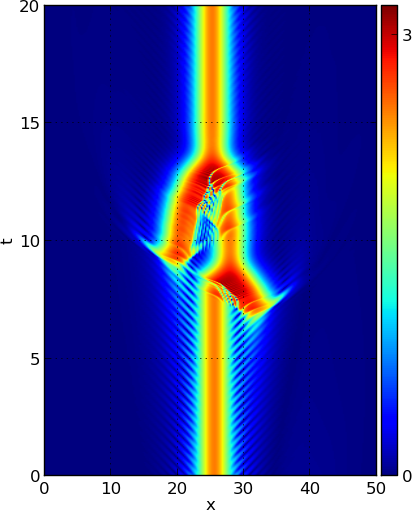
\includegraphics[width=0.33\textwidth]{asymmetricExplosion2}
  \caption{Three different types of soliton explosion: symmetric,
  asymmetric type 1, asymmetric type 2. $\mu = -0.1$. Color
  represents the magnitude of $A$.}
  \label{fig:explosionTypes}
\end{figure}
At present, no precursor to the explosion has been found and
it is unclear how the explosion frequency depends on the
system size and parameters. Also, you can see that
the center of mass of the localized
soliton stays unchanged under symmetric explosion and shifts left or right
under asymmetric explosion. Such a phenomenon is also observed in the
2-dimensional case \cite{CaCiDeBr12}.  So one of our goals of
undertaking this system is to calculate the diffusion coefficient
of the solition by cycle expansion. Recently,
people \cite{Descalzi10, Jaime2012, Jaime2013,
Akhmediev04, Orazio2011, CaCiDeBr12}
use different approximation schemes to explain
this phenomenon and and test their predictions by numerical experiments.
However, little has been shed on the unstable invariant solutions in this
system, nor their stability analysis.

On the other hand,
\CqcGL\ \eqref{eq:cqcgl1d} has three symmetries:
\begin{itemize}
\item  \textbf{translational symmetry}. $\tau_\ell A(x,t) = A(x+\ell,t)$.
\item \textbf{phase invariance}. $\rho_\phi A(x,t) = e^{i\phi}A(x,t)$.
\item \textbf{symmetric reflection}.$R_s A(x,t) = A(-x, t)$.
\end{itemize}
Previous research does not leverage the continuous/discrete symmetries
of this system. We will
simplify the state space by reducing the symmetries and then apply
cycle expansion theory.
